\chapter{Opis projektnog zadatka}
		
		%\textbf{\textit{dio 1. revizije}}\\
		
		U današnje vrijeme većina ljudi živi užurbanim tempom, stoga svaki slobodan trenutak žele iskoristiti za odmor i rekreaciju. Mnoge ljude privlači boravak na svježem zraku te kao rezultat toga, sve više ljudi izabire planinarenje kao jednu od brojnih mogućnosti koje im se nude. Međutim, planinari pri odabiru rute za svoje planinarske izlete često nemaju dovoljno informacija pa se koriste usmenom predajom i nagađanjima. Tako planinari, osobito planinari rekreativci, nailaze na različite probleme od kojih su najčešći krive informacije o stazama i rutama ili planinarski domovi bez odgovarajuće infrastrukture. Upravo zbog toga pokrenut je projekt čiji je cilj razvoj i evolucija programskog proizvoda, odnosno web aplikacije „Planinarski dnevnik“. Aplikacija će uvelike pomoći planinarima u organiziranju svojih planinarskih izleta, ali i ponuditi točne informacije o rutama na pojedinim izletima te povezati planinare poznanike u vlastitu planinarsku zajednicu. Osim toga, planinari će moći pretraživati i planinarske domove koji se nalaze na odabranim stazama, a za svaki dom će biti prikazane koje pogodnosti on nudi (prenoćište, topao obrok, pitka voda, struja, grijanje itd.). \\
		
		Opseg projektnog zadatka sadrži sve aktivnosti i zadatke koji su vezani uz izradu aplikacije. Za početak se radi analiza aplikacije kako bi se utvrdilo koliko će okvirno vremena biti potrebno za izradu određene komponente aplikacije. U tome dobrim dijelom pomažu dnevnik sastajanja i dnevnik aktivnosti koji služe kao kontrolne točke pomoću kojih se vidi ide li daljnji napredak aplikacije u dobrom smjeru. Na tim sastancima prisutni su asistenti koji su stručnjaci za ovo područje i svojim savjetima višestruko pomažu timu. \\
		
		Za izradu „Planinarskog dnevnika“ predviđen je vremenski period od 13 tjedana, odnosno jednog fakultetskog semestra. Radi se analiza interesnih sudionika s namjerom da se što točnije odredi broj korisnika koji će biti zainteresirani za korištenje aplikacije. Svrha same aplikacije je educirati studente na fakultetu pa shodno tome ne postoje troškovi prilikom izrade iste. Krajnji cilj je potpuno razvijena aplikacija s ispravnom programskom potporom koja sadrži sve zahtijevane komponente i podržava rad više korisnika u stvarnom vremenu. Kada je navedeno postignuto, aplikacija je spremna za lansiranje na tržište kako bi se korisnici mogli njome služiti.\\
		
		Aplikacija „Planinarski dnevnik“ zasigurno će biti najzanimljivija planinarima kojima je i namijenjena, ali također i mnogobrojnim ustanovama poput planinarskih domova kojima će omogućiti promociju u širem krugu korisnika. Potencijalno bi moglo doći do povećanja prihoda kao rezultat brojnih usluga koje planinarski domovi pružaju, ali i poboljšanja kvalitete istih sukladno s porastom broja planinara koji ih posjećuju. Proširit će se opseg planinarskog turizma na manje poznata područja tako što će postati vidljiva širem krugu korisnika aplikacije. Također, korisnost ove aplikacije odrazit će se na HGSS (Hrvatska gorska služba spašavanja) koja će efikasnije saznati sve potrebne informacije o kretanju i ruti planinara u slučaju nesreće ili nestanka. Evidentno je da će se područje pretrage znatno smanjiti jer će planinar unaprijed odrediti rutu svojeg kretanja.\\
		
		Pokretanjem aplikacije svakom korisniku prvotno će biti dodijeljena uloga \underbar{Gost} koja omogućava pretraživanje postojećih planinarskih domova prema dostupnoj infrastrukturi (pitka voda, hrana, prenoćište...) ili
		pretraživanje planinarskih staza prema zahtjevnosti, trajanju ili duljini. Za sve daljnje aktivnosti korisnik će se morati registrirati u sustav tako što će u predloženu formu za registraciju unijeti osobne podatke:
		\begin{packed_item}
			\item ime
			\item prezime
			\item e-mail
			\item lozinku
			\item sliku (opcionalno)
			\item nešto više o sebi (opcionalno)
			\item datum rođenja (opcionalno)
			\item mjesto stanovanja (opcionalno)	
		\end{packed_item}
	 
		Nakon što se korisnik registrira dodijelit će mu se uloga \underbar{Planinar} i moći će pristupiti vlastitom profilu. Omogućit će mu se pregled i uređivanje osobnih podataka te u krajnjem slučaju uklanjanje korisničkog računa. Planinar može uspostaviti odnos s ostalim registriranim planinarima tako što šalje zahtjeve za "prijateljstvom", odnosno zahtjeve za dodavanje na popis vlastite planinarske zajednice, ali i na način da ostale članove svoje planinarske zajednice pozove na određeni događaj. Prema unaprijed određenom predlošku dopušta se stvaranje vlastitih planinarskih staza kao i vlastitih događaja. Uz to se nudi i mogućnost ocjenjivanja stvorenih planinarskih staza kao i prijava netočnih ili nepreciznih informacija vezanih uz pojedine staze, što može biti od velike koristi svim planinarima, osobito početnicima koji na osnovu najviše ocjene mogu odabrati svoju željenu stazu. Na naslovnici će biti prikazane objave prijatelja planinara, a na zidu obavijesti će biti vidljiv popis prihvaćenih ili odbijenih pozivnica te prihvaćenih ili odbijenih zahtjeva za prijateljstvom. Nudi se i svrstavanje planinarske staze ili doma na popis željenih te dodavanje ranije odrađenih planinarskih staza u osobnu arhivu. Dolaskom planinara na cilj evidentirat će se njihovo prisutstvo, a nakon određenog broja osvojenih vrhova ostvarit će pravo na bedž kao jednu vrstu motivacije za još veću aktivnost u budućnosti. \\
		
		Svaki planinar ima priliku dobiti ulogu \underbar{Dežurnog planinara} tako što tu ulogu zatraži od administratora. Nakon što bilo koji registrirani planinar posjeti određeni planinarski dom, dobiva potvrdu o posjetu od planinara koji je zadužen za taj planinarski dom, tzv. dežurnog planinara.\\
		
		Sustav nadgleda \underbar{Administrator} koji ima najveće ovlasti. Ukoliko neki korisnik (planinar) ne poštuje pravila ponašanja, administrator ima pravo obrisati njegov korisnički račun. On će zaprimati primjedbe od korisnika na određene staze te će ovisno o količini netočnih informacija odlučiti hoće li staza biti izmijenjena ili uklonjena s liste. Također će odobravati zahtjeve za dežurnog planinara i dodijeliti ga određenom planinarskom domu. Time se sprječava ponavljanje istih pogrešaka u budućnosti i aplikacija će biti sve točnija i vjerodostojnija. 
		
		
		\section{Primjeri sličnih rješenja}
		Slične implementacije rješenja projektnog zadatka već postoje. Na području Republike Hrvatske možemo izdvojiti iduće: 
		\begin{packed_enum}
			\item Kao prvi primjer navodimo aplikaciju \textbf{eHPS} koja je razvijena pod pokroviteljstvom Hrvatskog planinarskog saveza. Njena svrha je omogućavanje korisniku efikasno pretraživanje podataka o svim planinarskim domovima, kućama i skloništima koji postoje na području Republike Hrvatske. Također pruža uslugu iščitavanja i proučavanja podataka o svim kontrolnim točkama i dosad otvorenim planinarskim obilaznicama.
			\item Druga slična aplikacija je \textbf{infoHPS} koja pruža uslugu pretraživanja postojećih planinarskih udruga koje su članice Hrvatskog planinarskog saveza. Za svaku traženu udrugu omogućuje prikaz informacija bitnih za korisnika poput naziva, OIB-a udruge, email-a itd. 
		\end{packed_enum}
	
			\begin{figure}[H]
			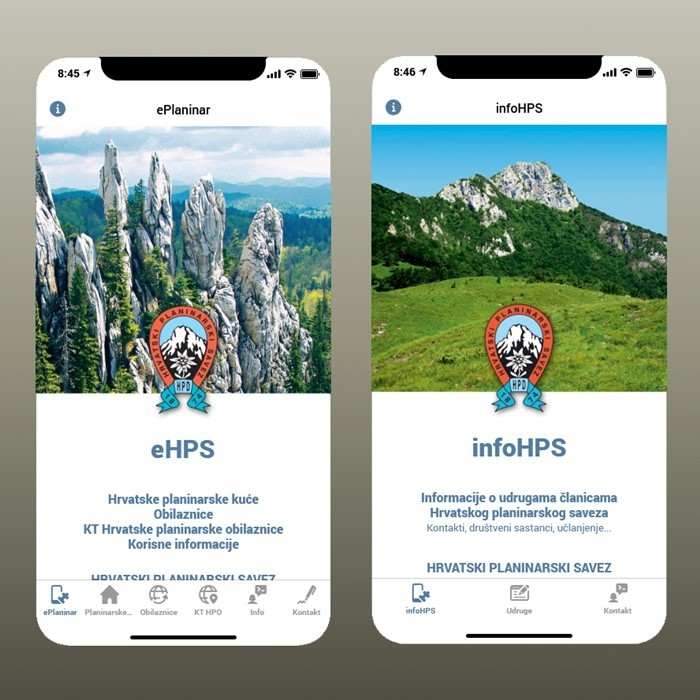
\includegraphics[scale=0.5]{slike/HPS.jpg} %veličina slike u odnosu na originalnu datoteku i pozicija slike
			\centering
			\caption{Primjeri sličnih aplikacija - eHPS i infoHPS}
			\label{fig:slične aplikacije}
			\end{figure}
	
		Na području SAD-a aplikacija \textbf{Mountain project} nudi korisnicima pretraživanje postojećih planinarskih ruta, čitanje novosti i razmjenjivanje poruka između prijavljenih korisnika.
			
			\begin{figure}[H]
				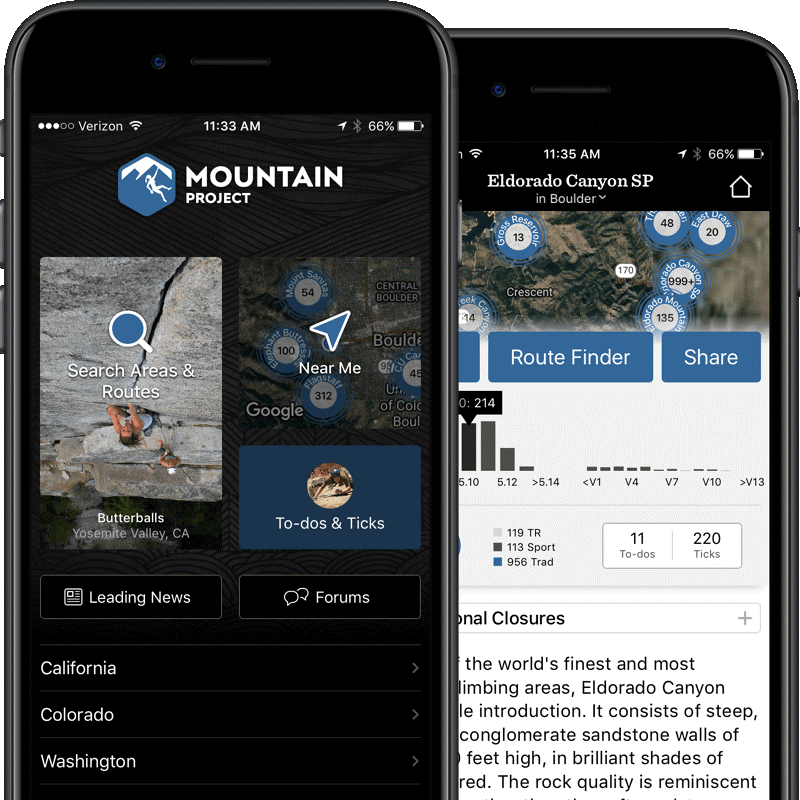
\includegraphics[scale=0.3]{slike/mountainproject.png} %veličina slike u odnosu na originalnu datoteku i pozicija slike
				\centering
				\caption{Primjer slične aplikacije - Mountain Project}
				\label{fig:slične aplikacije}
			\end{figure}
		
		\section{Moguće nadogradnje projektnog zadatka}
		Postoje brojne funkcionalnosti kojima bi se mogla nadograditi i proširiti postojeća aplikacija te ispraviti eventualne nepravilnosti. Jedna od mogućnosti je implementacija „Chat-a“ za razmjenu poruka i iskustava među planinarima koji pripadaju istoj planinarskoj zajednici. Uz to, mogao bi se dodati i neformalni forum gdje bi svi planinari mogli podijeliti svoja iskustva, doživljaje i preporuke ostatku planinarske zajednice. Aplikacija bi trebala imati i mogućnost instaliranja na pametne satove koji su postali neizostavni dio planinarske i sportske opreme.  Također bi bilo korisno kad bi korisnici odlaskom na naslovnu stranu aplikacije mogli vidjeti aktualne novosti, događanja iz planinarskog svijeta te preporučene izlete u skladu s vremenskim uvjetima. Svaki planinar mora imati odgovarajuću opremu prije nego što krene na izlet pa bi oglašavanje i prodaja planinarske opreme bio izvrstan dodatak aplikaciji. Registrirani planinar bi mogao postaviti oglas sa slikom i opisom opreme koju prodaje, cijenom i lokacijom na kojoj se nalazi. Sadašnja verzija aplikacije sadrži unesene izlete namijenjene većinom za pješačke rute. U budućnosti bi se aplikacija mogla proširiti dodavanjem ruta za bicikliranje ili čak i skijanje. Još jedna od korisnih funkcionalnosti bila bi uvođenje uloge „planinarski dom“. Uloga bi planinarskim domovima omogućila kreiranje vlastitih događaja kao što su organizirani izleti, zabave i slično. 
		
		\eject
		
	